%%%%%%%%%%%%%%%%%%%%%%%%%%%%%%%%%%%%%%%%%%%%%%%%%%%%%%%%%%%%%%%%%%%%%%%%%%%%%
%%
%% This file provides a template that can be used in concert with the
%% ohio-etd class to generate an electronic thesis or dissertation which
%% meets the formatting requirements at Ohio University.
%%
%% To use the template, copy this file (template.tex) and ohio-etd.cls into
%% the same directory and edit this template as required.  Reference
%% ohio-etd.pdf for additional instructions on using this class.
%%
%%%%%%%%%%%%%%%%%%%%%%%%%%%%%%%%%%%%%%%%%%%%%%%%%%%%%%%%%%%%%%%%%%%%%%%%%%%%%


%% Load the class.  Available options are: numbered, pdftex, cmfont,
%% singlespacetables, draft, 11pt, 12pt, leqno, and fleqn

\documentclass[numbered,pdftex]{ohio-etd}


%% Other packages that may be of use.  Delete or comment out (using a
%% percent sign in the first column) if they are not desired.  Reference
%% the corresponding documentation for more information on how to use these
%% packages.

\usepackage[square,sort&compress,numbers]{natbib} % Provides formatting for
                                                  % citations
\usepackage{textcomp} % Provides math symbols that can be used in text mode
\usepackage{amssymb}  % Provides additional AMS math symbols.  Note that
                      % amsmath is loaded as part of the ohio-etd class
\usepackage{bm}       % Provides bold-faced math symbols
\usepackage{booktabs} % Provides improved table formatting
\usepackage{dcolumn}  % Provides table columns aligned at decimal points
\usepackage{multirow} % Provides table elements spanning multiple rows
\usepackage{graphicx} % Standard package to incorporate graphics
\usepackage[printonlyused]{acronym} % Provides a method for incorporating 
                                    % acronyms and building an acronym list
\usepackage{listings}
\lstdefinelanguage{myC}{
  language=C,
  basicstyle=\ttfamily\singlespacing,
  showspaces=false,              
  showstringspaces=false,        
  showtabs=false,    
  tabsize=2,                      % sets default tabsize to 2 spaces
  captionpos=b,                   % sets the caption-position to bottom
  breaklines=true,                % sets automatic line breaking
  breakatwhitespace=false,
  escapeinside={\%*}{*)},        
  keywordstyle=\bfseries\color{black},    % keyword style
  numberstyle=\tiny\color{gray},
%  numbers=left,
%  frame=single,                  % adds a frame around the code
%  rulecolor=\color{black},
%  stepnumber=1,                 
%  numbersep=5pt,                
%  backgroundcolor=\color{white}, 
%  commentstyle=\color{dkgreen},  % comment style
%  stringstyle=\color{mauve},     % string literal style
}
% A version of the above myC, but without singlespacing
\lstdefinelanguage{myinlineC}{
  language=myC,
  basicstyle=\ttfamily
}
\renewcommand{\ttdefault}{pcr}    % enables bold monospaced font
\lstdefinelanguage[x86gasm]{Assembler}[x86masm]{Assembler}{%
,basicstyle=\ttfamily\singlespacing
,morekeywords={rax,rbx,rcx,rdx,rip,rdi,rsi,rsp,subq,decl,movq
              ,movl,xorl,imull,popq,popl,pushl}%
,morekeywords=[2]{.file,.section,.string,.text,.globl,.cfi_startproc
                 ,.cfi_def_cfa_offset,.cfi_endproc,.size,.ident}%
}
\lstdefinelanguage{Coq}{
,morekeywords={match,end,Definition,Inductive,Lemma,Theorem,Record,
               Variable,Hypothesis,Section,End,case,of,if,then,else,Let,
               is,let,in,do,return,with,Extract,Constant,Inlined,Inline,
               Extraction,Fixpoint,Program,Function,Fix,type,Class,for}%
,keywordstyle=\bfseries\color{MidnightBlue}
,basicstyle=\sffamily
,columns=fullflexible
,numberstyle=\tiny\color{gray}
%,escapeinside={@}{@}
,literate=
    {:=}{{$\defeq\;$}}1
    {<-}{{$\leftarrow\;$}}1
    {=>}{{$\Rightarrow\;$}}1
    {->}{{$\rightarrow\;$}}1
    {<->}{{$\leftrightarrow\;$}}1
    {<==}{{$\leq\;$}}1
    {\\/}{{$\vee\;$}}1
    {/\\}{{$\land\;$}}1
    {fun\ }{{$\lambda$\ }}1
    {forall}{{$\forall$}}1
    {exists}{{$\exists$}}1
    {Z}{{$\mathbb{Z}$}}1
    {Z0}{{$\mathbb{Z}_0$}}1
    {<=}{{$\leq\;$}}1
    {>=}{{$\geq\;$}}1
    {<>}{{$\neq\;$}}1
    {Q}{{$\mathbb{Q}$}}1                    
}

\lstset{language=Coq, basicstyle=\fontencoding{T1}}
\usepackage{natbib}
\usepackage[usenames,dvipsnames,svgnames,table]{xcolor} 

\graphicspath{{images/}} % Allows graphics files to be stored in a
                          % separate directory



%% Required front matter definitions

\degree    {MS}              % MS, MA, MCTP, or PhD
\graduation{August}{2020}    % May, August, or December 

\title     {Formalized Generalization Bounds for Perceptron-Like Algorithms}
\author    {Robin J.}{Kelby} 

\advisor   {Gordon Stewart}{Assistant Professor of Electrical Engineering and Technology}
\dean      {Mei Wei}{Dean, Russ College of Engineering and Technology}

\program   {Computer Science}            
\department{School of Electrical Engineering and Computer Science} 
\college   {Russ College of Engineering and Technology}   
\abstract  {Machine learning algorithms are integrated into many aspects of daily life. However, research into the correctness and security of these important algorithms has lagged behind experimental results and improvements. My research seeks to add to our theretical understanding of the Perceptron family of algorithms, which includes the Kernel Perceptron, Budget Kernel Perceptron, and Description Kernel Perceptron algorithms. \\ In this thesis, I will describe three variants of the Kernel Perceptron algorithm and provide both proof and performance results for verified implementations of these algorithms written in the Coq Proof Assistant. This research employs generalization error, which bounds how poorly a model may perform on unseen testing data, as a guarantee of performance with proofs verified in Coq. These implementations are also extracted to the functional language Haskell to evaluate their generalization error and performance results on real and synthetic data sets. }

%% Optional front matter definitions.  Delete or comment out if not needed

%\coadvisor {Coadvisor's Full Name}{Coadvisor's Full Title}

%\dedication{%\pagebreak
%\hspace{0pt}
%\vfill
%\emph{\begin{center} 
%\end{center}}
%\vfill
%\hspace{0pt}}



\acknowledgments{Acknowledge later}
%% If you prefer to provide "acknowledgements" instead (note the added "e"
%% between the "g" and the "m") then add the "e" in the macro name so that
%% it reads "\acknowledgements".}

%% Additional "lists" can be added to the end of the front matter using the
%% \addlistof macro.  For example:
%\addlistof{Symbols}{Insert your list of symbols here or comment out this line.}
%% Note that the command "\input{symbols}" can be used if the symbol list is
%% contained in a separate file called "symbols.tex"}

%\addlistof{Acronyms}{Insert your list of acronyms here or comment out this line}
%% Use "\input{acronyms}" if the acronym list is in a separate file called
%% "acronyms.tex".  Note that the formatting generated by the acronym package
%% can be forced into singlespaced text by inserting "\setlength\itemsep{0pt}
%% \setlength\parskip{0pt}" into the "acronym" environment.} 

% \notables  % Prevent a list of tables from being created
% \nofigures % Prevent a list of figures from being created

\begin{document} 

\makefrontmatter    % Creates all of the front matter pages.

%% Body of the text follows, using \chapter, \section, \subsection,
%% \subsubsection, \paragraph, and \subparagraph to generate the
%% section headings.  For convenience, it may be useful to break the
%% full document into separate files, perhaps divided by chapters.  In
%% that case, the files would be loaded here using "\input{filename}"

\chapter{Introduction}

The field of machine learning research has advanced rapidly in the past decade. Machine learning describes the class of computer programs that automatically learn from experience, often employed for classification, recognition, and clustering tasks. One of the classic problems in machine learning is digit recognition to classify handwritten numbers automatically. Computers have historically struggled to interpret handwritten information because handwriting can vary drastically between writers. While humans can be taught to read as well as learn to read on their own, handwriting recognition can be challenging for computers to accomplish. Several datasets have been created to provide a common source of handwritten digit data so that the performance of different machine learning algorithms can be directly compared. For example, the MNIST dataset \cite{LBBH98} is one of the primary datasets for computers to learn how to classify handwritten digits into the numbers 0-9. This dataset allows researchers to compare the performance of multiple models, trained and tested on the same data, but using different machine learning algorithms. Some systems have achieved a near-perfect performance on the MNIST dataset for the problem of handwritten digit classification, and this technology is valuable for processing documents, such as ZIP codes on letters sent through the U.S. Postal Service \cite{MKB17}.
\\Increasingly, machine learning has been heavily integrated into our daily lives. As described by the authors of ``Social media big data analytics", social media companies such as Facebook, Twitter, and YouTube learn from our digital data in order to serve individuals with targeted information and often advertising \cite{GHHA19}. Retailers track customer purchases to learn about individuals' habits and entice them with specific offers and coupons. The pages we visit, profiles we create, and products we buy are used to predict our future actions and monetize our attention. This kind of task would be almost impossible for a human to complete, due to the vast amounts of data involved per person or account. In addition to social media, retailers, and advertisers, machine learning techniques are also being employed in critical systems, such as healthcare and infrastructure, where failure can lead to the loss of time, money, and lives. Research to evaluate the use and oversight of machine learning algorithms \cite{Var16} has shown that there are few existing safety principles and regulations for critical systems that rely on machine learning components. Machine learning drives more than websites and commerce; its algorithms are also responsible for the well-being and safety of people around the world, and regulation has largely not caught up with machine learning advances.
\\The details of machine learning differ from algorithm to algorithm, but for most methods, machine learning algorithms learn models from training data to encode the program's knowledge. Models consist of learned parameters, which represent different kinds of data depending on the encoding of the model, and hyperparameters, a small number of variables directly specified by the programmer that may control the speed of training or other high level details. Models tend to be complex, and can require thousands or millions of learned parameters for high accuracy on a given problem. Learned models are able to take a new piece of data as input and produce a result or judgment from that data. For the recognition of handwritten digits, the input to the model is the handwritten digit, and the output is the classification of that digit as a number from 0-9.
\\The development of new machine learning algorithms or advances in training and validation techniques tends to be experimentally driven in most applications. New or finely tuned configurations for internal components can lead to increased accuracy and efficiency or decreased training time compared to other algorithms for a specific problem or dataset. Small refinements to algorithms and hyperparameters can have enormous impacts on training time, model size, and performance on unseen testing data. Because of the complexity of the models produced by many machine learning algorithms, many new papers published in the field describe results found through experimentation, as opposed to examining the underlying theory responsible for these advances. Additional research in understanding the theory behind machine learning may help to understand why some techniques are better suited for some problems than others, as well as potential avenues for exploration.
\\Finding errors in machine learning algorithms or models can be very difficult. With thousands or millions of parameters learned by the computer, not specified by the programmer, algorithms can easily get stuck in small, local solutions instead of finding the optimal solution. For example, gradient descent is an algorithm tasked with finding the lowest, or global, minimum of a multi-dimensional hillside with many peaks and valleys. Through many iterations, gradient descent travels downward along the gradient until a place is reached where descent is no longer possible. If the algorithm cannot find a deeper valley, this depth is returned as the overall solution. However, gradient descent can fail to find the global solution when the hyperparameters are not tuned correctly by the programmer or deeper valleys take too long to find, which can occur for nonconvex optimization problems. Techniques have been developed to mitigate the limitations of gradient descent, such as momentum, but the programmer usually has to experiment with multiple techniques to achieve peak performance. Additionally, few machine learning algorithms have theoretical properties that can be verified, such as a theorem that a learning algorithm will always terminate or find the global solution. Research into verifying machine learning to produce models with optimal behavior is limited due to these difficulties.
\\One way to increase our knowledge in the theory of machine learning is to verify the correctness of machine learning algorithms through mathematical, machine-checked proofs. Formal verification often employs proof assistants, such as Coq, which allow for the integration of proofs with software specifications and implementations. Mathematical proofs in Coq are guaranteed to be as valid as the proof assistant itself and the correctness of the specifications and theorems proved. Proofs are implemented as portable programs, which allows for others to verify proofs independently. Because proofs and implementations are written in the same environment, the proofs directly correspond to the implementation verified. The Coq environment also provides libraries containing both implementations of data structures and proofs to aid in the development of verified systems.
\\Researchers have used the Coq proof assistant to verify many different software systems and prove correctness properties. The CompCert compiler for the C language \cite{Ler09} is the first realistic verified compiler, proving that the behavior of a C program compiled with CompCert will not be changed in the transformation of compilation. Verified compilers ensure that the executable program produced by the compiler does not contain errors produced in compilation. For safety-critical applications, executables created by a verified compiler are more secure than executables created by unverified compilers. Another verified system written in Coq is Verdi \cite{WWP15}, a framework for specifying and implementing distributed systems with tolerance for node faults. In a network of computers, connections can be dropped, packets lost or sent out of order, and nodes can fail or restart. Verdi allows the programmer to specify the fault conditions their distributed system should be resilient against, and the Verdi system itself mechanizes much of the proof process and code extraction for deployment in real-world networks. Distributed system software written with Verdi has been verified to handle faults and errors that may occur. Finally, the CertiKOS project \cite{GSC16} has developed several microkernels with security properties and proofs of correctness, including mC2, a verified concurrent microkernel. Operating systems allocate memory and computer resources and must defend against malicious processes. Coq has been used to specify and verify a diverse range of algorithms, data structures, and applications beyond these three projects.
\\In this thesis, I will describe my additions to the verification framework MLCert \cite{MLC}. MLCert provides software tools and libraries in the Coq proof assistant for verified machine learning in Coq, such as generic definitions and proofs for machine learning algorithms, example algorithms such as the Perceptron, and extensions for the implementation and training of neural networks. Building on the Perceptron implementation and existing proofs in MLCert, I present a verified implementation of the Kernel Perceptron algorithm, as well as two variants on the Kernel Perceptron algorithm: a Budget Kernel Perceptron and a Description Kernel Perceptron. Background information for this thesis is provided in Chapter 2, with an introduction to the Perceptron and Kernel Perceptron algorithms, a more extended discussion of the challenges and tactics of machine learning verification, and motivation for the Budget Kernel Perceptron and Description Kernel Perceptron algorithms. Chapter 3 describes the methodology for implementing these algorithms in Coq. The proofs for these implementations and their performance results are detailed in Chapter 4. Finally, future work and conclusions are discussed in Chapter 5.


\chapter{Background}\label{BackgroundChapter}
This chapter aims to provide necessary background information in order to understand the remainder of this thesis. Sections \ref{PerceptronSection} and \ref{KernelPerceptronSection} describe the Perceptron algorithm and its descendant, the Kernel Perceptron algorithm. Next, the challenges and methods of formal verification of machine learning are discussed in sections \ref{MLVerificationSection} and \ref{MLCertFrameworkSection}. Finally, modifications of the Kernel Perceptron algorithm, such as Budget Kernel Perceptrons in section \ref{BudgetKernelPerceptronSection} and Description Kernel Perceptrons in section \ref{DescriptionKernelPerceptronSection}, are detailed as improvements for the Kernel Perceptron.
\section{The Perceptron Algorithm}\label{PerceptronSection}
The Perceptron algorithm was initially published in 1957 by Frank Rosenblatt. Highly influential in the early growth and development of the field of artificial intelligence, the Perceptron \cite{Ros57} provided one of the first methods for computers to iteratively learn to classify data into discrete categories. In order to classify $n$-dimensional data, the Perceptron learns a weight vector with $n$ parameters as well as a bias term. Both the weight vector and bias consist of positive integers greater than or equal to zero which encode a linear hyperplane separating two or more categories in $n$-dimensional space.

\begin{figure}
    \caption{Perceptron Pseudocode}
    \label{PerceptronPseudo}
    \begin{lstlisting}
Definition Perceptron (w:Params) (epochs:nat) (training_set:list (Label * Data)) :
for i in epochs:
    for j in size(training_set):
        (example, true_label) = training_set[j]
        predict = Predict(example, w)
        if predict != true_label:
            w = Update(w, training_set[j]).
    \end{lstlisting}
\end{figure}

The most basic Perceptron algorithm has the following steps. Before training, each parameter in the weight vector $w$ is initialized to zero. The algorithm consists of two nested loops, as shown by the pseudocode in Figure \ref{PerceptronPseudo}. For this algorithm, we require the weight vector, the number of epochs, and the training set as input. The training set consists of labeled training examples, where the label is either 0 or 1. The outer loop uses the number of epochs to control the number of iterations over the entire training set. The inner loop executes for every training example in the training set and has two main steps. First, the $n$-dimensional data inside the training example and the weight vector are used to calculate the Perceptron's predicted label for this example, without using the training example's true label. The calculation for Perceptron prediction is shown in pseudocode in Figure \ref{PerceptronPredictPseudo} takes as input the weight vector and a single training example to produce a predicted label for the given example.

\begin{figure}
    \caption{Perceptron Prediction Pseudocode}
    \label{PerceptronPredictPseudo}
    \begin{lstlisting}
Definition Predict (example:Data) (w:Params):
    (bias, weight) = w 
    bias + dot_product(weight, example).
    \end{lstlisting}
\end{figure}

The true label and the calculated predicted label are then compared. If both labels are the same, the Perceptron correctly classified this training example. However, if the predicted label is different, the weight vector is updated using the example to improve classification over time. This update is the second step of the inner loop.
\\The Perceptron algorithm is powerful despite its simplicity. However, there are limitations to the Perceptron's classification. The Perceptron cannot classify data that is not linearly separable with 100\% accuracy, such as points classified by the exclusive-OR function, a binary operator that returns TRUE when its two inputs are the opposite of each other. Despite the simplicity of exclusive-OR, the Perceptron cannot produce a model, or linear hyperplane, such that all the points classified by exclusive-OR as TRUE are also classified by the Perceptron as TRUE, and all the points classified by exclusive-OR as FALSE are also classified by the Perceptron as FALSE. The Perceptron can achieve at best 75\% accuracy for the exclusive-OR function. This restriction on the Perceptron caused the first AI Winter, a severe decline in artificial intelligence research, due to unreasonable expectations for the Perceptron in fields where data is not linearly separable.
\\While the Perceptron is limited to classification of linearly separable data, the Perceptron Convergence Theorem states that the Perceptron is guaranteed to converge to a solution on linearly separable data. This property of the Perceptron algorithm was first proven on paper by Papert in 1961 \cite{Pap61} and Block in 1962 \cite{Blo62}. However, this proof was not verified by machine until 2017 through the work of Murphy, Gray, and Stewart \cite{MGS17} in the Coq proof assistant. 
\section{The Kernel Perceptron}\label{KernelPerceptronSection}
The Kernel Perceptron improved on the Perceptron algorithm with the introduction of the kernel trick by Aizerman, Braverman, and Rozoner \cite{ABR64}. Using kernel functions, the classification of the Perceptron can be expanded to include non-linearly separable data. There are four main modifications for the Kernel Perceptron: prediction, kernel functions, parameter space, and weight vector update. Prediction for the Kernel Perceptron uses kernel functions to produce non-linear hyperplanes instead of linear hyperplanes. Because of kernalization, the prediction function changes so that in addition to the weight vector $w$ and the current training example, the training set and training labels are required as well. The bias term is no longer necessary.

\begin{figure}
    \caption{Kernel Perceptron Prediction Pseudocode}
    \label{KernelPerceptronPredictPseudo}
    \begin{lstlisting}
Definition KernelPredict (example:Data) (w:KernelParams) 
        (training_set:list (Label * Data) (K:Kernel):
    for i in size(training_set):
        (label, data) = training_set[i]
        sum += w[i] * label * K(example, data)
    return sum.
    \end{lstlisting}
\end{figure}

In the pseudocode KernelPredict function shown in Figure \ref{KernelPerceptronPredictPseudo}, $K$ represents an arbitrary kernel function. Kernel functions form a class of functions that take two examples as input and produce a single value. By using non-linear kernel functions, the Kernel Perceptron can classify data that is not linearly separable. For example, the Kernel Perceptron can classify the exclusive-OR function with 100\% accuracy
using a quadratic kernel. 
\\By using kernel functions in prediction, the parameters used by the Kernel Perceptron have different cardinality compared to the parameters of the Perceptron. The Kernel Perceptron requires one parameter per training example for its classification, regardless of the dimensionality of the data. Therefore, the size of the weight vector is dependent on the size of the training set. 
\\Finally, the weight vector update for the Kernel Perceptron is somewhat different from that of the Perceptron. When a training example is misclassified by the Kernel Perceptron, its parameter is incremented and the rest of the weight vector is unchanged. The full Kernel Perceptron algorithm is shown in Figure \ref{KernelPerceptronPseodo}.

\begin{figure}
    \caption{Kernel Perceptron Pseudocode}
    \label{KernelPerceptronPseodo}
    \begin{lstlisting}
Definition KernelPerceptron (w:KernelParams) (epochs:nat)
        (training_set:list (Label * Data)) (K:Kernel):
for i in epochs:
    for j in size(training_set):
        (example, true_label) = training_set[j]
        predict = KernelPredict(example, w, training_set, K)
        if predict != true_label:
            w = Update(w, j).
    \end{lstlisting}
\end{figure}

The Kernel Perceptron improves upon the Perceptron, but the Kernel Perceptron has its own limitations. The size of the parameter space for the Kernel Perceptron limits its usefulness in applications where memory is at a premium, as the size of the weight vector is dependent on the number of training examples, not the dimensionality of the training data. Also, the Kernel Perceptron, due to the use of kernel functions, is not guaranteed to converge to a solution or terminate, unlike the Perceptron algorithm. This means that the Perceptron Convergence Theorem cannot be used to prove the correctness of an implementation of the Kernel Perceptron.
\section{Approaches to Machine Learning Verification}\label{MLVerificationSection}
Verifying machine learning algorithms is a difficult problem in software engineering. Machine learning algorithms can produce thousands or millions of parameters in their models, which interact to classify data. The learning process for machine learning models can be tedious for humans to trace, and the model parameters generated during training are often not human-interpretable for manual verification of correctness. The authors of \cite{BF16} describe how machine learning researchers do not agree on a standard definition of what human interpretability is or how models should be able to be interpreted by humans. Interpretability varies between algorithms and tends to be more difficult for neural algorithms, including the Perceptron family of algorithms. Some formal verification in the field of machine learning has been performed, as shown by \cite{TD05}, but many algorithms have not been verified correct. Even for implementations with paper proofs of correctness, few have been proven correct by machine.
\section{MLCert Framework}\label{MLCertFrameworkSection}
To facilitate the verification of machine learning algorithms, Bagnall and Stewart developed MLCert \cite{BS19}, an open-source tool built in the Coq proof assistant. MLCert employs generalization error to prove correctness for machine learning algorithms. Generalization error, as described by Levin, Tishby, and Solla \cite{LTS90}, is an important indicator for the robustness of a machine learning model; algorithms with low generalization error can generalize from the training examples used in training to correctly classify unseen examples from the same domain of data in testing. Instead of trying to verify the model directly, MLCert verifies the generalization bounds for machine learning implementations built in its framework. Bounds on the generalization error indicate that an algorithm has bounds on mistakes made during testing, and the size of the parameter space contributes heavily to the tightness of the generalization bounds. Verified generalization bounds guarantee worst-case performance for a model. Previous work in the MLCert framework \cite{BS19} has resulted in an implementation of the Perceptron algorithm with proofs to verify its generalization bounds. However, to the best of our knowledge, no one has implemented the Kernel Perceptron in Coq or formally proven its correctness of generalization bounds using machine-checked proofs.
\\The parameter space for the Kernel Perceptron is dependent on the number of training examples. This means that, as compared to the Perceptron algorithm, the Kernel Perceptron has very loose generalization bounds due to the increased size of the parameter space. The tightness of the generalization bounds matters because tighter bounds provide a stronger guarantee for performance. To tighten the generalization bounds of the Kernel Perceptron, one approach is to limit the number of parameters.
\section{Budget Kernel Perceptron Algorithms}\label{BudgetKernelPerceptronSection}
Budget Kernel Perceptrons are a family of algorithms which modify the Kernel Perceptron to limit the size of the parameters for the model while minimizing the impact on the accuracy of the model. Budget Kernel Perceptrons are often employed in areas where computer memory or resources are at a premium, and their modifications are customized for the requirements of their field. One strategy for Budget Kernel Perceptrons is to keep a set number of training examples for classification called support vectors, which specific rules for updating this set over time to maintain its size as the classification boundary changes. For the base Kernel Perceptron algorithm described in Section \ref{KernelPerceptronSection}, every training example is a support vector. An example of a budget update rule is described in the article ``Tracking the best hyperplane with a simple budget Perceptron'', where the authors describe an update procedure where one support vector is selected at random for each replacement \cite{CCBG07}. Another update rule is to always select the oldest support vector for replacement, as this support vector may no longer be necessary for correct classification. 
\\Other strategies minimize the impact of removed support vectors through more creative means. Dekel, Shalev-Shwartz, and Singer present the Forgetron, where each support vector is ``forgotten'' over time by decreasing its impact on the model, which means that there is always an oldest support vector to be removed with the least influence on the model \cite{DSSS07}. The authors of \cite{CKS03} compute the distance of each support vector from the classification hyperplane and remove the support vector with the greatest distance. Finally, the Projectron and Projectron++ algorithms described by \cite{OKC09} store both a support set and a projection onto the support set to reduce the overall size of the model. All these methods balance model size with increased classification error compared to the base Kernel Perceptron.
\\Of these studies, only Cramer, Kandola, and Singer \cite{CKS03} provide paper proofs of their Budget Kernel Perceptron's generalization bounds. The nature and function of Budget Kernel Perceptrons complements our research in proving generalization error for machine learning algorithms. By implementing a Budget Kernel Perceptron, the bounds on the size of the parameter space can improve the bounds on generalization error compared to the base Kernel Perceptron algorithm.
\section{Description Kernel Perceptrons}\label{DescriptionKernelPerceptronSection}
In contrast to Budget Kernel Perceptrons, another method of encoding the Kernel Perceptron parameters involves description-length bounds. During training, the Kernel Perceptron will make the set number of mistakes, bounded by some value $L$. Using $L$, the number of support vectors is less than or equal to the number of mistakes, which will always be less than or equal to the size of the training set. This method requires a record of every misclassification made during training. Only training examples that were misclassified are included in the set of support vectors and used to calculate the hyperplane.
\\Description-length bounds describe the process of training, as each misclassification is recorded in order to produce and change the hyperplane. Instead of fixing the size of the support vectors on an arbitrary value, description-length bounds alow for every misclassification to be represented, while excluding training examples that are never misclassified and therefore not essential for the model. The generalization error for a Kernel Perceptron using description-length bounds is dependent on the number of misclassifications, which provides a bound on the size of the parameter space.
\section{Chapter Summary}\label{BackgroundChapterSummarySection}
This chapter summarizes the background of this thesis, discussing the Perceptron and Kernel Perceptron algorithms, as well as variants of the Kernel Perceptron algorithm with improved generalization bounds. Chapter 3 will next describe my extensions to the MLCert framework to implement three Kernel Perceptron algorithms: the base Kernel Perceptron algorithm, a Budget Kernel Perceptron, and a Description Kernel Perceptron, with generalization proofs for each implementation written in Coq.

\chapter{Methods}\label{MethodsChapter}
Blurb about what this chapter is about
\section{Structure of Perceptron Implementations in MLCert}\label{MLCertStruct}
\section{Kernel Perceptron Coq Implementation}\label{KPCoqImp}
\section{Budget Kernel Perceptron Coq Implementation}\label{KPBCoqImp}
\section{Description Kernel Perceptron Coq Implementation}\label{KPDCoqImp}
\section{Chapter Summary}\label{MethodsChapterSummarySection}
 
\chapter{Proofs and Experimental Results}\label{ResultsChapter}
The results of my research consist of proofs and experimental performance for the implementations described in Chapter \ref{MethodsChapter}. This chapter consists of two sections, one for generalization proofs and the other describing extraction and performance. The Kernel Perceptron generalization proofs can be found in subsection \ref{KPProofs}. Subsection \ref{KPBProofs} provides the Budget Kernel Perceptron generalization, and the Description Kernel Perceptron generalization is located in subsection \ref{KPDProofs}. In Section \ref{HaskellExtractionPerformance}, the extraction directives for the three implementations are detailed in subsection \ref{DetailsHaskellExtraction} which transform the Coq implementations to Haskell modules. Subsections \ref{SyntheticResults}, \ref{IrisResults}, \ref{SonarResults} describe the testing methodology for three datasets that were used to evaluate the experimental generalization error and analyze the runtime of training and testing each implementation. Finally, in subsection \ref{ResultsDiscussion}, the trends and results seen across datasets and implementations are outlined. The conclusions and future work for this research follow in Chapter \ref{ConclusionsChapter}.
\section{Generalization Proofs}\label{Proofs}
In the MLCert framework, much of the proof burden has been automated. For a new Learner representing a machine learning algorithm, there are two new lemmas that need to be proved. The first lemma proves the cardinality of the parameters used by the algorithm, which corresponds to the size of the parameter space. The second lemma applies the first in order to prove a generalization bound for the Learner as a whole. An example of the second lemma for a generic Learner is shown in Figure \ref{LearnerLemma}.

\begin{figure}
    \caption{Generalization Bound for a generic Learner}
    \label{LearnerLemma}
    \begin{lstlisting}
Lemma Learner_bound eps (eps_gt0 : 0 < eps) init : 
    @main A B Params Hypers Learner
      hypers m m_gt0 epochs d eps init (fun _ => 1) <=
    #|Params| * exp (-2%R * eps^2 * mR m).
    \end{lstlisting}
\end{figure}

The definition of main which is used in Figure \ref{LearnerLemma} can be found in the file ``learners.v''. Once main has been instantiated with the specifics of the Learner, such as its particular Params and Hypers, there are proofs in ``learners.v'' such as the lemma main\_bound which provide the machinery necessary to prove this inequality over the real numbers. As described by Bagnall and Stewart \cite{BS19}, MLCert uses Hoeffding's inequality, a type of Chernoff bound, to prove the generalization bound for a Learner. The value eps is the difference between expected accuracy and empirical accuracy, which is a probability between zero and one. The specific value of eps is chosen to ensure that the resulting bound is also a probability, as a bound greater than one is no longer useful for bounding generalization error. In the following subsections, the lemmas proving the generalization bounds for the Kernel Perceptron, Budget Kernel Perceptron, and Description Kernel Perceptron will be discussed.
\subsection{Kernel Perceptron Generalization Proofs}\label{KPProofs}
The bound for the Kernel Perceptron relies on the size of the parameter space. As proven in the lemma K\_card\_Params in the section KernelPerceptronGeneralization, the cardinality of the parameters for the Kernel Perceptron is shown in Equation \ref{KPParams}. This power of two is calculated by unfolding the definition of Params, which consists of the training set and a float array of size m. As all values are floating point numbers stored in 32 bits, the cardinality of a single floating point number is $2^{32}$. Therefore, as the dimensions of the training set are equal to m training examples multiplied by n dimensions, the cardinality of the training set is equal to $2^{m*n*32}$. The cardinality of a float array of size m is $2^{m * 32}$. 

\begin{equation} \label{KPParams}
 \#|Params| = 2^{(m*n*32 + m*32)}
\end{equation}

Kcard\_Params is central to the proof of the generalization bounds of the Kernel Perceptron in the lemma KPerceptron\_bound, which is defined in Figure \ref{KPLemma}. The generalization bound for the Kernel Perceptron is very loose, as growth in the size of the training set causes exponential growth in the generalization error. This limits the usefulness of the Kernel Perceptron's generalization bound, as a loose generalization bound provides few guarantees for performance or correctness. However, the Kernel Perceptron bound allows for comparison between this result and the generalization bounds for the Budget Kernel Perceptron and the Description Kernel Perceptron. 

\begin{figure}
    \caption{Generalization Bound for the Kernel Perceptron}
    \label{KPLemma}
    \begin{lstlisting}
Lemma Kperceptron_bound eps (eps_gt0 : 0 < eps) init : 
    @main A B Params KernelPerceptron.Hypers 
      (@KernelPerceptron.Learner n m KPsupport_vectors H K)
      hypers m m_gt0 epochs d eps init (fun _ => 1) <=
    2^(m*n*32 + m*32) * exp (-2%R * eps^2 * mR m).
    \end{lstlisting}
\end{figure}

\subsection{Budget Kernel Perceptron Generalization Proofs}\label{KPBProofs}
The Budget Kernel Perceptron has a similar bound on the cardinality of the parameter space. However, the parameter space for the Budget Kernel Perceptron is not dependent on m, the size of the training set, whatsoever. Instead, the parameter space relies on (S sv), which is the size of the support set. The successor of sv is used to denote the size of the support set so that the budget update procedure is always possible regardless of the value of sv, as there will be at least one support vector able to be replaced.
\\Like the Kernel Perceptron, the Budget Kernel Perceptron stores the support set and a float array. The float array is of size (S sv), so its cardinality is $2^{32 * (S sv)}$. The support set stores (S sv) training examples, which consist of one float value for each of the n dimensions of the data, plus a Boolean value for the label of the support vector. Therefore, the cardinality of each training example in the support set is $2^{1 + n * 32}$. The full cardinality of the Budget Kernel Perceptron Params is given in Equation \ref{KPBParams}. The lemma proving this bound is found in the section KernelPerceptronGeneralizationBudget, named Kcard\_Params\_Budget.

\begin{equation} \label{KPBParams}
 \#|Params| = 2^{((32*(S sv) + ((1 + n * 32)*(S sv))))}
\end{equation}

Figure \ref{KPBLemma} shows the lemma for the generalization bound of the Budget Kernel Perceptron, which uses Kcard\_Params\_Budget in its proof. Comparing the bound of the Budget Kernel Perceptron to the Kernel Perceptron, the overall structure of the two bounds is similar when the number of training examples is the same. However, because the support set can be significantly smaller than the number of training examples, the Budget Kernel Perceptron's bound is tighter than that of the base Kernel Perceptron. 

\begin{figure}
    \caption{Generalization Bound for the Budget Kernel Perceptron}
    \label{KPBLemma}
    \begin{lstlisting}
Lemma Kperceptron_bound_budget eps (eps_gt0 : 0 < eps) init : 
    @main A B Params KernelPerceptronBudget.Hypers 
      (@KernelPerceptronBudget.Learner n sv F K U)
      hypers m m_gt0 epochs d eps init (fun _ => 1) <=
    INR 2^((32*(S sv) + ((1 + n * 32)*(S sv)))) * exp (-2%R * eps^2 * mR m).
    \end{lstlisting}
\end{figure}

\subsection{Description Kernel Perceptron Generalization Proofs}\label{KPDProofs}

The generalization bound for the Description Kernel Perceptron is similar to that of the Budget Kernel Perceptron. First, we must define the cardinality of the parameter space used by the Description Kernel Perceptron. The parameters store a single float32 value paired with (S des) support vectors. The successor of des is used as the size of the support set, so that support vector replacement is always possible. Like with the Budget Kernel Perceptron, the cardinality of each support vector in the support set is $2^{1 + n * 32}$, which stores a single Boolean label as well as $n$ 32-bit floating point values. However, because there is not a float value for every support vector, only the cardinality of a single float32 must be added to the cardinality of the entire support set. The cardinality of the Description parameters is shown in Equation \ref{KPDParams}.

\begin{equation} \label{KPDParams}
 \#|Params| = 2^{((32 + ((1 + n * 32)*(S des))))}
\end{equation}

Figure \ref{KPDLemma} shows the generalization bound of the Description Kernel Perceptron in the lemma Kperceptron\_bound\_Des. This bound is similar to the bound of the Budget Kernel Perceptron, but is tighter because there is only one float32 value instead of a float32 value per support vector. This small difference means that if the budget is the same as the number of mistakes, the Description Kernel Perceptron will have a slightly tighter bound. 

\begin{figure}
    \caption{Generalization Bound for the Description Kernel Perceptron}
    \label{KPDLemma}
    \begin{lstlisting}
Lemma Kperceptron_bound_Des eps (eps_gt0 : 0 < eps) init : 
    @main A B Params KernelPerceptronDes.Hypers 
      (@KernelPerceptronDes.Learner n des F K)
      hypers m m_gt0 epochs d eps init (fun _ => 1) <=
    INR 2 ^ (32 + (1 + n * 32) * (S des)) * exp (-2%R * eps^2 * mR m).
    \end{lstlisting}
\end{figure}

\section{Haskell Extraction and Performance Experiments}\label{HaskellExtractionPerformance}
In order for the Coq implementations to be run, these implementations must be extracted to Haskell. The file ``extraction\_hs.v'' contains extraction directives for Haskell so that some Coq functions and data structures are extracted properly. The last Coq module for each implementation uses the extractible\_main definition, found in ``learners.v'', to also provide the necessary machinery that Learner.t relies on. The extracted Coq code is written to a Haskell file located in the directory hs/ in MLCert.
\\The extracted Haskell code for a machine learning algorithm does not contain code to initialize the system with training and testing data or functions to display accuracy and generalization error results to the user. Unverified Haskell drivers have been written for these implementations, which include the extracted Haskell code as a module. The Haskell drivers for the Kernel Perceptron implementations can also be found in the hs/KernelPerceptron/ directory.
\subsection{Details of Haskell Extraction}\label{DetailsHaskellExtraction}
The extraction directives for the Kernel Perceptron can be found in the section KPerceptronExtraction in the file ``kernelperceptron.v''. This section extracts the Kernel Perceptron to the Haskell file ``KPerceptron.hs'', a Haskell module that can be included by a Haskell driver program. This file is extracted to the two locations in MLCert where Haskell driver programs reside: hs/KernelPerceptron/ and hs/KernelPerceptron/timing\_drivers/. The Budget Kernel Perceptron and Description Kernel Perceptron each have their own extraction directives to extract ``KPerceptronBudget.hs'' and ``KPerceptronDes.hs'' to these same locations. 
\\There are four different kinds of Haskell driver programs for a variety of different purposes. All driver programs report the training accuracy, test accuracy, and generalization error for the dataset run by that driver. Several also print the model produced by training. The drivers are differentiated by their file names, which identify the purpose of the drivers.
\\``KPerceptronXOR.hs'' tests that the Kernel Perceptron using a quadratic kernel can classify the XOR function with 100\% accuracy. The linear kernel cannot be used because the XOR function is not linearly separable. The four samples for this function are specified in the driver, along with the quadratic kernel for the prediction function. When run, this driver demonstrates that the Kernel Perceptron behaves as expected with the quadratic kernel and is able to classify data that is not linearly separable. This is the only driver that uses nonlinear data and a nonlinear kernel function for prediction.
\\Each implementation has a driver that generates a new linearly separable dataset using a random number generator to test that the implementation can execute. These drivers have Test in their file names. After randomly generating $n$ floating point values between negative one and one, these values form the linear hyperplane used to produce labels for the training and test examples, which are randomly generated by the same process. These synthetic datasets test that the implementations have been set up correctly and can classify linear data. However, because the datasets are generated differently for each run of the program, these drivers cannot be used to compare implementations.
\\To compare the accuracy of an implementation on a specific dataset, each implementation has a driver which reads a dataset from files and performs training and testing. These drivers have RunFile in their file names. The drivers require that the input dataset be stored in two files, one containing the training set and the other containing the test set. The dataset files must also be formatted with one example per line and values separated by commas. The first value of the line must be a positive unique integer, which is used by the Kernel Perceptron to differentiate between the training examples for updates. The last value must be either True or False, corresponding to the label for the example. As long as the dataset files are formatted correctly, the driver will train and test on this dataset and report the accuracy and generalization error for this dataset. Only one dataset is run by this driver.
\\Finally, to time the execution of training and testing on a dataset, drivers with FileIO in their name read in one or more datasets. The FileIO drivers run training and testing five times and report the time in seconds. There are a total of 15 drivers to time all datasets, five for each implementation. The drivers do not time reading the dataset files and use the same format as the RunFile drivers. 
\\In the following subsections, I will detail my testing methodology on three datasets, two real datasets downloaded from the UCI Machine Learning Repository \cite{DG17} and a synthetic dataset created from randomly generated linear hyperplanes. The Iris Data Set \cite{Fis36} and Sonar Mines vs. Rocks Data Set \cite{SG88} were formatted to conform to be more easily read into the driver programs. Each of the following subsections describes the dataset under test, the experimental setup and drivers used, the calculated generalization error, and the timing results for training and testing.
\subsection{Synthetic Dataset Performance Results}\label{SyntheticResults}
A synthetic dataset was created specifically to test the performance of the Kernel Perceptron and its variants. There are 20 independent trials in this dataset with training and testing sets based on randomly generated data separated by a randomly oriented linear hyperplane. Each trial contains 1000 training examples and 1000 test examples, each with three dimensions. These datasets were created by recording and formatting the output of 20 runs of KPerceptronTest.hs. 
\\Because the Kernel Perceptron variants are all deterministic, the generalization error results were found using the RunFile driver for each implementation. All implementations ran for five epochs. The Budget Kernel Perceptron limited the size of the support set to 100 examples, 10\% of the training set, and the Description Kernel Perceptron was similarly limited to 100 mistakes. 
\\The generalization error of the three implementations is graphed in Figure \ref{SyntheticGenErrFig}. The Kernel Perceptron and Budget Kernel Perceptron have the same training and testing error for all 20 synthetic trials, while the Description Kernel Perceptron tends to have slightly worse training and testing accuracy and increased generalization error on some trials. The greatest observed generalization error is 1.4\% for the Description Kernel Perceptron in Trial 8.

\begin{figure}[h]\label{SyntheticGenErrFig}
 \caption{Synthetic Generalization Error}
 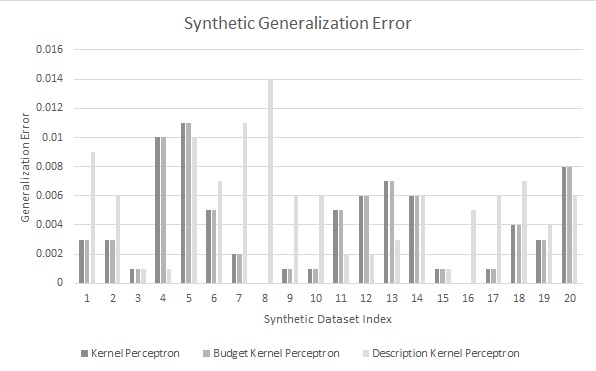
\includegraphics[scale=0.9]{SyntheticGenErr}
\end{figure}

Table \ref{tab:avesyntheticaccgen} provides statistics across the synthetic trials for average training and testing accuracy and generalization error, along with the 95\% confidence interval for each implementation. Because the Kernel Perceptron and Budget Kernel Perceptron had the same performance across all trials, their averages and confidence interval are the same. The Description Kernel Perceptron's averages reflect its tendency to have lower accuracy and increased generalization error, and its confidence interval is larger than the other two implementations. For many of these trials, the Description Kernel Perceptron would require several more mistakes to have the same performance as the Kernel Perceptron and Budget Kernel Perceptron.

\begin{table}[h!]
 \begin{center}
  \caption{Average Synthetic Generalization Error and Confidence Intervals}
  \label{tab:avesyntheticaccgen}
  \begin{tabular}{l|c|c|c}
  \textbf{ } & \textbf{KP} & \textbf{Budget KP} & \textbf{Description KP}\\
  \hline
  \textbf{Average Training Accuracy} & 98.61\% & 98.61\% & 96.915\%\\
  \textbf{Average Testing Accuracy} & 98.58\% & 98.58\% & 96.87\%\\
  \textbf{Average Generalization Error} & 0.39\% & 0.39\% & 0.565\%\\
  \textbf{95\% Confidence Interval} & 0.001435352 & 0.001435352 & 0.001539834\\
  \end{tabular}
 \end{center}
\end{table}

Using the generalization bounds as proven in Section \ref{Proofs}, the number of training examples, dimensionality of the data, and size of the support set can be input to determine if the observed generalization error compares to the calculated bound. Table \ref{tab:syntheticgencalc} shows the generalization bound for two values of eps, zero and one, as eps represents probability. Unfortunately, for both of these values, all the implementations have vacuous bounds far greater than one. With the settings used in the above experiments, the calculated generalization bounds are unable to be compared to the observed generalization error. 

\begin{table}[h!]
 \begin{center}
  \caption{Synthetic Generalization Bound Calculations}
  \label{tab:syntheticgencalc}
  \begin{tabular}{l|c|c|c}
  \textbf{ } & \textbf{KP} & \textbf{Budget KP} & \textbf{Description KP}\\
  \hline
  \textbf{Training Examples} & 1000 & 1000 & 1000\\
  \textbf{Dimensionality} & 3 & 3 & 3\\
  \textbf{Support Vectors} & 1000 & 100 & 100\\
  \textbf{eps = 0} & 6.90947E+38531 & 1.93617E+3883 & 4.20647E+2929\\
  \textbf{eps = 1} & 1.78025E+37663 & 4.98862E+3014 & 1.08381E+2061\\
  \end{tabular}
 \end{center}
\end{table}

Worse still is the fact that the Kernel Perceptron always produces vacuous bounds. Because all training examples are support vectors, the smallest possible training set is a single example. The smallest possible dimensionality of data is one dimensional. Therefore, the generalization bound for the smallest possible dataset of a single one-dimensional training example stored as a 32-bit floating point value is shown in Equation \ref{KPBoundBad}. This bound is calculated to be 1.84467E+19 for eps = 0 and 2.49650E+18 for eps = 1. The bound becomes even more vacuous as the dimensionality of the data and number of examples increases. Because of this, the Kernel Perceptron cannot be used to compare calculated generalization error to generalization error observed in experiments.

\begin{equation} \label{KPBoundBad}
 2^{(m*n*32 + m*32)} * e^{-2*eps^{2}*m} = 2^{(1*1*32 + 1*32)} * e^{-2*eps^{2}*1} = 2^{64}*e^{-2eps^{2}}
\end{equation}

To determine if the Budget Kernel Perceptron and Description Kernel Perceptron produce nonvacuous bounds, different support set sizes and values of eps were input into their generalization bounds. Fortunately, with the settings listed in Table \ref{tab:syntheticlimitedgen}, nonvacuous bounds were found for both variants. The synthetic dataset was used to evaluate the effect of a limited budget for the Budget Kernel Perceptron and a limited number of mistakes for the Description Kernel Perceptron. Both implementations have a generalization bound of about 9\% for a three-dimensional dataset containing one thousand training examples and two support vectors or mistakes for Budget and Description, respectively. To produce these values, eps must be set to 0.301 for the Budget Kernel Perceptron and 0.282 for the Description Kernel Perceptron. The generalization error produced by these implementations with limited budget and mistakes is graphed in Figure \ref{SyntheticGenErr2Fig}. Overall, the training and testing accuracy for both implementations is far lower than the accuracy produced with larger support sets, but the difference between training and testing accuracy remains small. The greatest observed generalization error observed for the Budget Kernel Perceptron is 5.7\% and for the Description Kernel Perceptron is 4.8\%, well below the 9\% calculated bound, which validates the theoretical bound proven in Coq for these implementations.

\begin{figure}[h]\label{SyntheticGenErr2Fig}
 \caption{Synthetic Generalization Error using Limited Budget and Mistakes}
 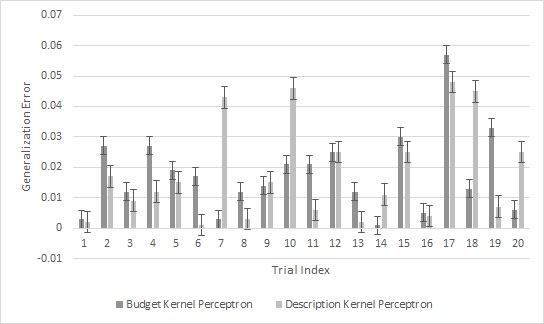
\includegraphics[scale=0.9]{SyntheticGenLimit}
\end{figure}

\begin{table}[h!]
 \begin{center}
  \caption{Synthetic Generalization Error and Confidence Intervals using Limited Budget and Mistakes}
  \label{tab:syntheticlimitedgen}
  \begin{tabular}{l|c|c}
  \textbf{ } & \textbf{Budget KP} & \textbf{Description KP}\\
  \hline
  \textbf{Training Examples} & 1000 & 1000\\
  \textbf{Dimensionality} & 3 & 3\\
  \textbf{Support Vectors} & 2 & 2\\
  \textbf{eps} & 0.301 & 0.282\\
  \hline
  \textbf{Calculated Bound} & 9.35\% & 9.10\%\\
  \textbf{Greatest Observed Generalization Error} & 5.7\% & 4.8\%\\
  \hline
  \textbf{Average Training Accuracy} & 76.89\% & 78.625\%\\
  \textbf{Average Testing Accuracy} & 76.6\% & 78.11\%\\
  \textbf{Average Generalization Error} & 1.79\% & 1.805\%\\
  \textbf{95\% Confidence Interval} & 0.005794861 & 0.007007097\\
  \end{tabular}
 \end{center}
\end{table}

The runtimes of the three implmentations were also evaluated to compare training and testing performance. The runtime for each trial was tested five times to determine average training and testing. Figure \ref{SyntheticKernelTiming} shows the synthetic timing results for the Kernel Perceptron. All runtimes were around 200 seconds, with little variation between trials. The averages for each trial and their 95\% confidence intervals are listed in Table \ref{tab:synthetictiming}.

\begin{figure}[p]\label{SyntheticKernelTiming}
 \caption{Kernel Perceptron Synthetic Timing}
 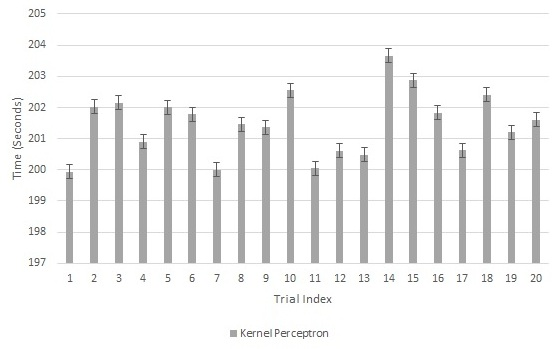
\includegraphics[scale=0.8]{KernelSyntheticTiming}
\end{figure}

The Budget Kernel Perceptron and Description Kernel Perceptron execute much faster than the Kernel Perceptron because their models are significantly smaller. Figure \ref{SyntheticBudgetDesTiming} shows the synthetic timing results for these two implementaitons. The Budget Kernel Perceptron took around 0.35 seconds to train and test, while the Description Kernel Perceptron took around 0.29 seconds. The Description Kernel Perceptron has the smallest model of the three implementations, causing it to have the fastest runtime. Table \ref{tab:synthetictiming} shows the averages and confidence intervals for each trial.

\begin{figure}[p]\label{SyntheticBudgetDesTiming}
 \caption{Budget and Description Kernel Perceptron Synthetic Timing}
 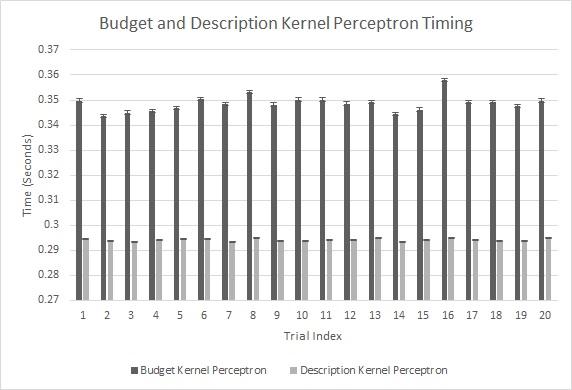
\includegraphics[scale=0.8]{BudgetDesSyntheticTiming}
\end{figure}

The confidence intervals for the Kernel Perceptron trials are much larger than the Budget and Description Kernel Perceptron trials because the runtimes for the Kernel Perceptron vary by seconds, as opposed to hundredths of seconds for the Budget and Description Kernel Perceptrons. These runtimes show that it is possible for the Budget and Description Kernel Perceptrons to have the same or similar accuracy as the Kernel Perceptron while training and testing in a shorter amount of time. 

\begin{table}[h!]
 \begin{center}
  \caption{Synthetic Average Runtimes and Confidence Intervals}
  \label{tab:synthetictiming}
  \begin{tabular}{l|c|c|c|c|c|c}
  \textbf{Trial} & \textbf{KP} & \textbf{95\% CI} & \textbf{Budget KP} & \textbf{95\% CI} & \textbf{Description KP} & \textbf{95\% CI}\\
  \hline
  \textbf{1} & 199.943 & 3.17258 & 0.3498 & 0.05499 & 0.2946 & 0.05606\\
  \textbf{2} & 202.025 & 2.44561 & 0.3436 & 0.05116 & 0.2938 & 0.05499\\
  \textbf{3} & 202.145 & 2.78125 & 0.345 & 0.05245 & 0.2932 & 0.05529\\
  \textbf{4} & 200.901 & 2.62953 & 0.3456 & 0.05263 & 0.294 & 0.05441\\
  \textbf{5} & 202.012 & 2.97056 & 0.3468 & 0.05351 & 0.2946 & 0.05557\\
  \textbf{6} & 201.786 & 2.46189 & 0.3504 & 0.05567 & 0.2944 & 0.05666\\
  \textbf{7} & 199.996 & 2.66681 & 0.3484 & 0.05175 & 0.2934 & 0.05422\\
  \textbf{8} & 201.455 & 3.07707 & 0.3532 & 0.05527 & 0.295 & 0.05440\\
  \textbf{9} & 201.362 & 2.92524 & 0.3482 & 0.05479 & 0.2936 & 0.05558\\
  \textbf{10} & 202.546 & 2.92950 & 0.3502 & 0.05332 & 0.2938 & 0.05452\\
  \textbf{11} & 200.051 & 2.58570 & 0.3502 & 0.05332 & 0.2942 & 0.05432\\
  \textbf{12} & 200.609 & 3.10256 & 0.3486 & 0.05215 & 0.294 & 0.05537\\
  \textbf{13} & 200.479 & 3.28990 & 0.3492 & 0.05331 & 0.2948 & 0.05647\\
  \textbf{14} & 203.655 & 3.41870 & 0.3444 & 0.05226 & 0.2934 & 0.05323\\
  \textbf{15} & 202.866 & 4.18980 & 0.3462 & 0.05384 & 0.294 & 0.05489\\
  \textbf{16} & 201.827 & 3.75820 & 0.358 & 0.05232 & 0.295 & 0.05587\\
  \textbf{17} & 200.627 & 3.80374 & 0.3492 & 0.05333 & 0.2942 & 0.05528\\
  \textbf{18} & 202.409 & 3.09442 & 0.3492 & 0.05381 & 0.2938 & 0.05450\\
  \textbf{19} & 201.203 & 2.51938 & 0.3476 & 0.05410 & 0.2938 & 0.05646\\
  \textbf{20} & 201.605 & 2.93406 & 0.3498 & 0.05351 & 0.295 & 0.05442\\
  \end{tabular}
 \end{center}
\end{table}

\subsection{Iris Dataset Performance Results}\label{IrisResults}
The Iris Dataset \cite{Fis36} contains 150 examples of four-dimensional data which represents 50 members each of three Iris species: Iris Setosa, Iris Versicolour, and Iris Virginica. Iris Setsosa is linearly separable from Iris Versicolour and Iris Virginica when Iris Versicolour and Iris are combined into a single class. This dataset is not divided into a training set and a testing set, which is required for determing generalization error as the difference between training and testing accuracy. To divide this dataset into a training set and a testing set, a random number generator was used to place each example either into the training set or the testing set. Two splits were used for this division, one with roughly 50\% training examples (77) and 50\% testing examples (73), and another with roughly 75\% training examples (113) and 25\% testing examples (37). These ratios were chosen to see if an increased number of training examples also increases the training and testing accuracy.

\begin{table}[p]
 \begin{center}
  \caption{Iris 50/50 Dataset Observed and Calculated Generalization Error}
  \label{tab:iris50gencalc}
  \begin{tabular}{l|c|c|c}
  \textbf{ } & \textbf{Kernel Perceptron} & \textbf{Budget KP} & \textbf{Description KP}\\
  \hline
  \textbf{Training Examples} & 77 & 77 & 77\\
  \textbf{Testing Examples} & 73 & 73 & 73\\
  \textbf{Dimensionality} & 4 & 4 & 4\\
  \textbf{Support Vectors} & 77 & 7 & 7\\
  \hline
  \textbf{Training Accuracy} & 100\% & 100\% & 100\%\\
  \textbf{Testing Accuracy} & 100\% & 100\% & 100\%\\
  \textbf{Generalization Error} & 0\% & 0\% & 0\%\\
  \hline
  \textbf{eps = 0} & 3.08721E+3036 & 6.76217E+271 & 1.07728E+214\\
  \textbf{eps = 1} & 4.05710E+2969 & 8.88660E+204 & 1.41572E+147\\
  \end{tabular}
 \end{center}
\end{table}

\begin{table}[p]
 \begin{center}
  \caption{Iris 75/25 Dataset Observed and Calculated Generalization Error}
  \label{tab:iris75gencalc}
  \begin{tabular}{l|c|c|c}
  \textbf{ } & \textbf{Kernel Perceptron} & \textbf{Budget KP} & \textbf{Description KP}\\
  \hline
  \textbf{Training Examples} & 113 & 113 & 113\\
  \textbf{Testing Examples} & 37 & 37 & 37\\
  \textbf{Dimensionality} & 4 & 4 & 4\\
  \textbf{Support Vectors} & 113 & 11 & 11\\
  \hline
  \textbf{Training Accuracy} & 100\% & 100\% & 100\%\\
  \textbf{Testing Accuracy} & 100\% & 100\% & 100\%\\
  \textbf{Generalization Error} & 0\% & 0\% & 0\%\\
  \hline
  \textbf{eps = 0} & 4.19104E+5442 & 1.33083E+533 & 6.23051E+436\\
  \textbf{eps = 1} & 2.96325E+2969 & 9.40956E+434 & 4.40525E+338\\
  \end{tabular}
 \end{center}
\end{table}

Once each training example was divided into separate training and testing files, each file was further formatted to replace the original labels of the dataset with Boolean values. Iris-setsosa was replaced with True, and both Iris-versicolour and Iris-virginica were replaced with False. A unique integer identifier was also added to the front of each example to conform to the specifications for file IO. With these preprocessing steps, the Iris data could be run by the Kernel Perceptron variants.
\\The generalization error results for the two Iris datasets were found using the RunFile driver for each implementation. All implementations ran for five epochs. The Budget Kernel Perceptron limited the size of the support set 10\% of the training set, and the Description Kernel Perceptron was similarly limited to 10\% of the size of the training set for the number of mistakes. 
\\The results for the 50/50 split of the Iris dataset are shown in Table \ref{tab:iris50gencalc}. All implementations had perfect training and testing accuracy, with no generalization error. However, none of the implementations had nonvacuous bounds for this dataset, as no setting of eps produced a bound less than one. The results for the Iris 75/25 split are shown in Table \ref{tab:iris75gencalc}. All implementations again had perfect training and testing accuracy, with no generalization error, and no implementation had nonvacuous bounds.
\\The timing results for the Iris datasets are shown in Figure \ref{IrisTiming}. As with the synthetic dataset, the Kernel Perceptron took significantly longer to train and test than the Budget and Description Kernel Perceptrons, with the Description Kernel Perceptron slightly faster to train and test than the Budget Kernel Perceptron. Table \ref{tab:iristabtiming} presents average runtimes and confidence intervals for the Iris datasets.

\begin{figure}[h]\label{IrisTiming}
 \caption{Iris Data Set Timing}
 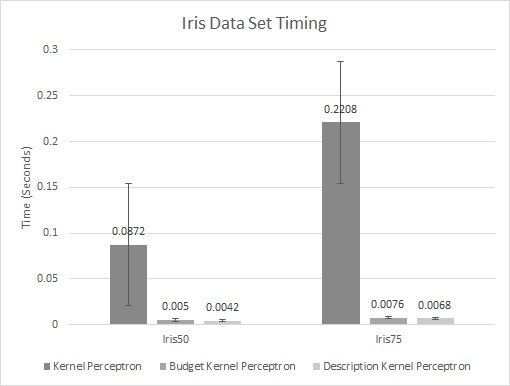
\includegraphics[scale=0.8]{IrisTiming}
\end{figure}

\begin{table}[h!]
 \begin{center}
  \caption{Iris Average Runtimes and Confidence Intervals}
  \label{tab:iristabtiming}
  \begin{tabular}{l|c|c|c|c|c|c}
  \textbf{Trial} & \textbf{KP} & \textbf{95\% CI} & \textbf{Budget KP} & \textbf{95\% CI} & \textbf{Description KP} & \textbf{95\% CI}\\
  \hline
  \textbf{Iris 50/50} & 0.0872 & 0.00342 & 0.005 & 0.00392 & 0.0042 & 0.00431\\
  \textbf{Iris 75/25} & 0.2208 & 0.00563 & 0.0076 & 0.00462 & 0.0068 & 0.00501\\
  \end{tabular}
 \end{center}
\end{table}

\subsection{Sonar Mines vs. Rocks Dataset Performance Results}\label{SonarResults}
The Sonar Mines vs. Rocks Dataset contains 208 examples of 60-dimensional data, representing sonar pings of either underwater explosive mines or roughly cylindrical rocks. This dataset is linearly separable. Like the Iris dataset, the Sonar dataset is not divided into a training set and testing set. Using the same method as the Iris dataset, two Sonar datasets were created with a roughly 50/50 split training and testing (116/92) and a roughly  75/25 split (157/51). The Sonar datasets were further preprocessed by adding a unique integer identifier to the front of each example and changing the labels from M to True and R to False. 
\\The values for each example in the original Sonar dataset are decimals ranging from zero to one. Based on Perceptron training in \cite{MGS17}, which stated that on the full dataset, their Perceptron took over 275,000 epochs to converge to a solution. Due to limitations on my machine used for performance experiments, it was not realistic to run my implementations for more than 10,000 epochs. Because of this limitation, the Sonar dataset was normalized from values from zero to one to values between negative one and one to center the examples closer to the zero vector used at the start of training. The normalized data files were used for the generalization error and timing experiments described below. 
\\Again, the generalization error results were found using the RunFile driver for each implementation. All implementations ran for 10,000 epochs. The Budget Kernel Perceptron was limited to 10\% of the training set and the Description Kernel Perceptron to 10\% of the training set as the number of mistakes.
\\The results for the 50/50 split of the Sonar dataset are shown in Table \ref{tab:sonar50gencalc} and for the 75/25 split are in Table \ref{tab:sonar75gencalc}. Only the Kernel Perceptron had results with higher than about 50\% accuracy for both Sonar Datasets. The results for the Budget Kernel Perceptron and Description Kernel Perceptron were disappointing due to the fact that the Sonar datasets violate their underlying assumptions. To produce a model with high accuracy, thousands of misclassifications must be made to incrementally move the hyperplane. Because the dataset contains a maximum of just 208 examples, variants that rely on making a number of mistakes significantly smaller than the number of training examples are bound to have poor performance. The accuracies of the Budget and Description Kernel Perceptron only increase when the number of misclassifications or support vectors is set to the minimum necessary, which means that such a setting will have much worse generalization error compared to the Kernel Perceptron. The Sonar datasets also do not produce nonvacuous bounds due to the size of the training set and the dimensionality of the data.

\begin{table}[ht]
 \begin{center}
  \caption{Sonar 50/50 Dataset Observed and Calculated Generalization Error}
  \label{tab:sonar50gencalc}
  \begin{tabular}{l|c|c|c}
  \textbf{ } & \textbf{Kernel Perceptron} & \textbf{Budget KP} & \textbf{Description KP}\\
  \hline
  \textbf{Training Examples} & 116 & 116 & 116\\
  \textbf{Testing Examples} & 92 & 92 & 92\\
  \textbf{Dimensionality} & 60 & 60 & 60\\
  \textbf{Support Vectors} & 116 & 11 & 11\\
  \textbf{Epochs} & 10,000 & 10,000 & 10,000\\
  \hline
  \textbf{Training Accuracy} & 100\% & 55.17\% & 55.17\%\\
  \textbf{Testing Accuracy} & 69.57\% & 51.09\% & 51.09\%\\
  \textbf{Generalization Error} & 30.43\% & 4.08\% & 4.08\%\\
  \hline
  \textbf{eps = 0} & 6.66773E+68162 & 1.06512E+6467 & 4.98653E+6370\\
  \textbf{eps = 1} & Would not compute & 1.86671E+6366 & 8.73934E+6269\\
  \end{tabular}
 \end{center}
\end{table}

\begin{table}[ht]
 \begin{center}
  \caption{Sonar 75/25 Dataset Observed and Calculated Generalization Error}
  \label{tab:sonar75gencalc}
  \begin{tabular}{l|c|c|c}
  \textbf{ } & \textbf{Kernel Perceptron} & \textbf{Budget KP} & \textbf{Description KP}\\
  \hline
  \textbf{Training Examples} & 157 & 157 & 157\\
  \textbf{Testing Examples} & 51 & 51 & 51\\
  \textbf{Dimensionality} & 60 & 60 & 60\\
  \textbf{Support Vectors} & 157 & 15 & 15\\
  \textbf{Epochs} & 10,000 & 10,000 & 10,000\\
  \hline
  \textbf{Training Accuracy} & 84.08\% & 54.14\% & 54.78\%\\
  \textbf{Testing Accuracy} & 82.35\% & 50.98\% & 50.98\%\\
  \textbf{Generalization Error} & 1.73\% & 3.16\% & 3.8\%\\
  \hline
  \textbf{eps = 0} & 7.18772E+92254 & 4.71762E+8818 & 6.49060E+8683\\
  \textbf{eps = 1} & Would not compute & 2.01955E+8682 & 2.77855E+8547\\
  \end{tabular}
 \end{center}
\end{table}

The timing results for the Sonar Datasets are given in Table \ref{tab:sonartabtiming}. These results were found by running 10,000 epochs for each implementation, and the confidence intervals for each implementation are also listed.

\begin{table}[ht]
 \begin{center}
  \caption{Sonar Average Runtimes and Confidence Intervals}
  \label{tab:sonartabtiming}
  \begin{tabular}{l|c|c|c|c|c|c}
  \textbf{Trial} & \textbf{KP} & \textbf{95\% CI} & \textbf{Budget KP} & \textbf{95\% CI} & \textbf{Description KP} & \textbf{95\% CI}\\
  \hline
  \textbf{Sonar 50/50} & 1045.839 & 1.49470 & 79.0278 & 2.06799 & 66.1688 & 1.28507\\
  \textbf{Sonar 75/25} & 2121.471 & 6.43889 & 138.6656 & 4.08308 & 121.6616 & 3.08207\\
  \end{tabular}
 \end{center}
\end{table}

\subsection{Discussion of Generalization Error and Timing Results}\label{ResultsDiscussion}
\section{Chapter Summary}\label{ResultsChapterSummarySection}
These results from the implementations of the Kernel Perceptron, Budget Kernel Perceptron, and Description Kernel Perceptron demonstrate that the generalization error for the Kernel Perceptron can be improved through limiting the size of the support set or placing a limit on the number of mistakes made during training. The conclusions drawn from these results are described in Chapter \ref{ConclusionsChapter}, along with a discussion of future work to be done in the field of machine learning verification.

\chapter{Conclusions}\label{ConclusionsChapter}

%% The \references command marks the point where the bibliography will
%% be inserted.  In the example below, the BibTeX commands are
%% inserted into the macro definition, but one could also manually
%% enter the bibliography entries if desired.
\references{
  %ETD does not define a particular required bibliography style.
  %They DO require entries to end in a period UNLESS they end in a URL
  %or DOI AND that DOIs be set in the same font as everything else.
  %I have modified the alphaurl style file, to conform to these requirements.
  \bibliographystyle{alphaurl_etd}   
  \bibliography{kpthesis} 
}

%\appendix           % Indicates the transition from chapters to appendices.  
                    % Subsequent 

%\chapter{An Appendix}
%\section{A Section in the Appendix}

\end{document}
